\chapter{Results}\label{Sec:Results}

\section{Maximal Representative Subsample}

Although model learning and performance evaluation in a supervised setting are well understood \cite{hastie}, the availability of unlabeled data gives additional optionsand also presents new challenges.
for relating training samples to test data. To further reduce the variance of the error estimate, each class is sampled with approximately equal proportions in both datasets, a technique called stratification. 

The two-stage model is conceptually simpler than the integrated model, and may in some cases have the greatest practical utility. The main advantage compared to the integrated model is that regularization parameters can be tuned without prior knowledge by cross-validation. Another advantage of the two-stage model is that in the second stage, after the example-specific weights have been derived, virtually any learning mechanism can be employed to produce the final classifier from the weighted training sample. This comes at the cost of only a marginal loss of performance compared to the integrated model. The integrated and two-step logistic regression and exponential models and kernel mean matching perform similarly well.

\begin{table}[ht]
    \begin{center}
		\captionsetup{width= 430pt}
            {\footnotesize
            \begin{tabular}{l|cccccccccc}
                \hline \hline
                           &  TP Rate & FP Rate & Precision & Recall & F-Measure & ROC Area & PRC Area & Class \\
                \hline
                      & 0.000 & 0.000 & ? & 0.000 & ? & 0.500 & 0.130 & GBS &\\
                      & 1.000 & 1.000 & 0.870 & 1.000 & 0.931 & 0.500 & 0.870 & GESIS &\\
                \hline \hline
		 W. Avg. & 0.870 & 0.870 & ? & 0.870 & ? & ? & 0.500 & 0.774 &
            \end{tabular}}
        \caption{Some descriptive statistics of location and dispersion for 2100 observed swap rates for the period from February 15, 1999 to March 2, 2007. Swap rates measured as 3.12 (instead of 0.0312). See Table \ref{Tab:DescripStatsRawDataDetail} in the appendix for more details.}
\label{Tab:DescripStatsRawData}
\end{center}
\end{table}

Estimating positive class prior with One-Class SVMs. trying to estimate a function f which is positive on S and negative on the complement. The dataset that you use for training can contain all or mostly normal cases. Typically, the SVM algorithm is given a set of training examples labeled as belonging to one of two classes. An SVM model is based on dividing the training sample points into separate categories by as wide a gap as possible, while penalizing training samples that fall on the wrong side of the gap. The SVM model then makes predictions by assigning points to one side of the gap or the other. Therefore, in one-class SVM, the support vector model is trained on data that has only one class, which is the “normal” class. It infers the properties of normal cases and from these properties can predict which examples are unlike the normal examples.  Predictions from the One-Class SVM are uncalibrated scores that may be possibly unbounded. be sure to normalize scores if you are comparing models based on different algorithms.

\begin{figure}[ht]
	\begin{center}
		\captionsetup{width= 400pt}
		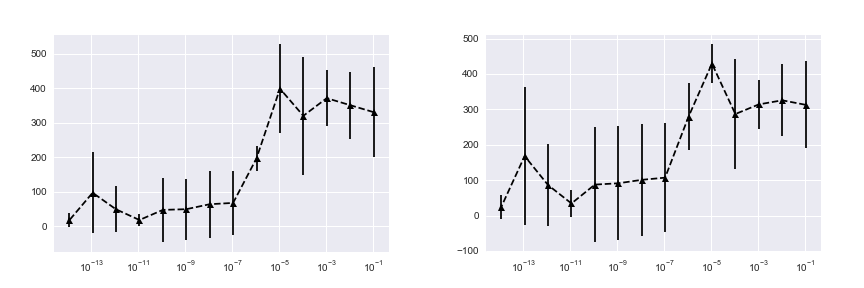
\includegraphics[scale=0.50,angle=0]{fig/occfigure}
		\label{occ}
		\caption{Using the One-Class SVM and its ability to capture the fraction of positive. Tuning parameter \(nu\) that controls the trade-off between the fraction of non-representative samples and the number of support vectors in one-class SVM. More than 0.73 of GBS (right) are classified as representative with high confidence (low sdt) for the optimal value \(nu = 10^{-5}\).}
	\end{center}
\end{figure}

\begin{figure}[ht]
\centering
		\captionsetup{width= 400pt}
   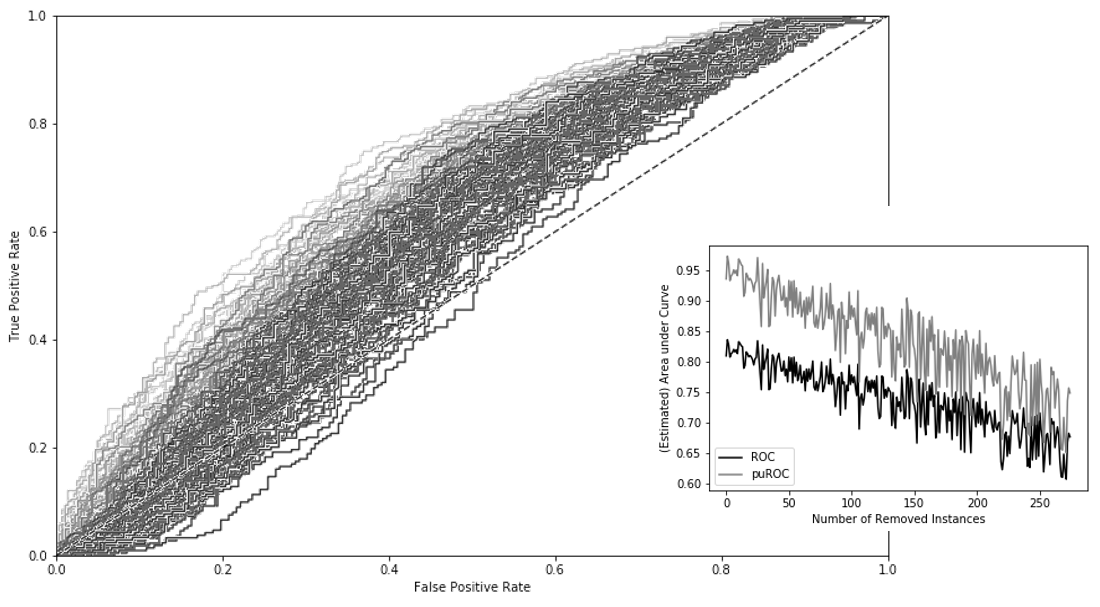
\includegraphics[scale=0.48,angle=0]{fig/res1}
\caption{ROC and puROC evaluation. An AUROC of approximately \(\frac{1}{2}\) implies that there is no more evidence for covariate shift.}
   \label{fig:Ng1} 
\end{figure}

\begin{figure}[ht]
\centering
\begin{subfigure}[b]{0.8\textwidth}
   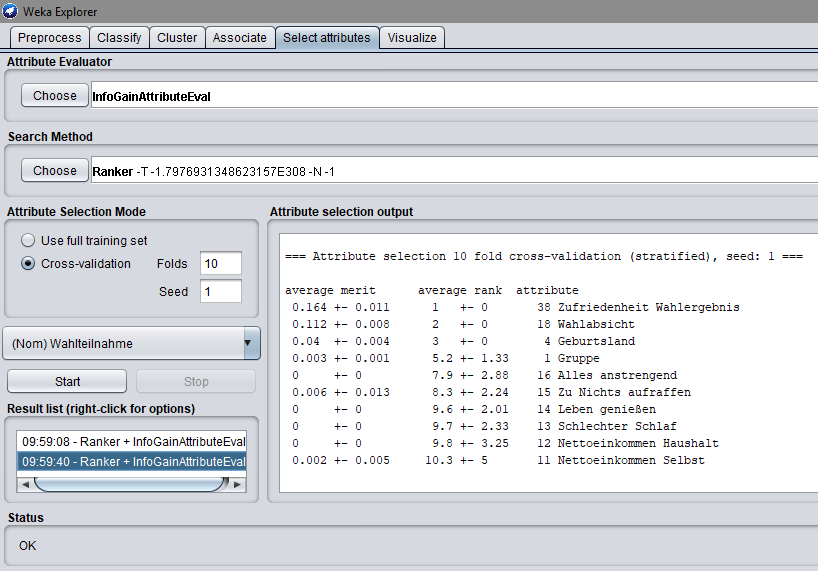
\includegraphics[scale=0.55,angle=0]{fig/weka_gbs}
   \label{fig:Ng1} 
\end{subfigure}
\begin{subfigure}[b]{0.8\textwidth}
\vspace{0.55cm}
   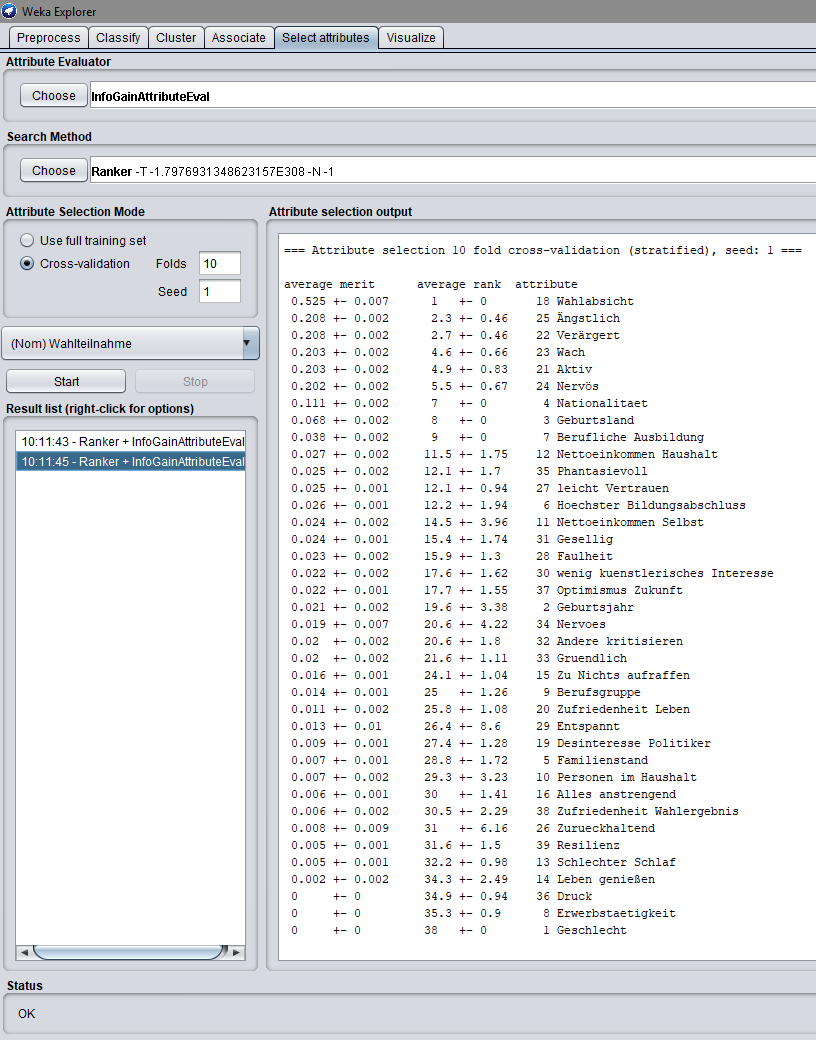
\includegraphics[scale=0.55,angle=0]{fig/weka_gesis}
   \label{fig:Ng2}
\end{subfigure}
\vspace{0.35cm}
\captionsetup{width= 400pt}
\caption{Feature importance in GBS (n=579) and GBS MRS (n=280) for classification of political participation "Wahlteilnahme". In modelling a political participation process, algorithms approximate the likelihood of a person going to vote on election day. Ideally, for every instance with unknown political interest and willingness to participate, there is enough data of people of similiar demographics, socioeconomics and psychological traits to generalize from.}
\end{figure}

\section{Future Work}

Many different adaptations, statistics, and experiments have been left for the future due to lack of time, i.e. data matching and transformation with real data have been very time consuming. Controlled environments are needed to observe the behavior of the proposed algorithm.

For one thing, future work concerns deeper analysis of the proposed sampling method, in particular, experiments on synthezised data. The Synthetic Minority Over-sampling TEchnique (SMOTE \cite{smote}) is a very popular oversampling method that creates synthetic minority class instances. The SMOTE instances are linear combinations of two similar instances from the minority class (\(x\) and \(x^{R}\)) and are defined as: \(s = x + u (x^{R} - x) \) with \(0 \geq  u \geq 1\). \(x^{R}\) is randomly chosen among the \(k\) nearest neighbors of \(x\) belonging to the minority class. SMOTE can be used to validate the MRS procedure by simulating the problem at hand.

Specific regions in the feature space are first over-sampled using SMOTE, before they are under-sampled by MRS. Experiments with multiple such synthesized data, with oversampling ratio ranging from high to low, might support the proposed procedure with greater evidence. The initial data sets are then compared to the result sets. GESIS is particularly well suited to artificially recreate the initial problem as visualized in Figure 5.1. It is only necessary to try to avoid giving the synthesized data properties that makes it possible for a learning algorithm to distinguish synthesized from non-synthesized example. This mechanism would for instance aid to compare classification results more easily.

\begin{figure}[ht]
	\begin{center}
\vspace{0.5cm}
		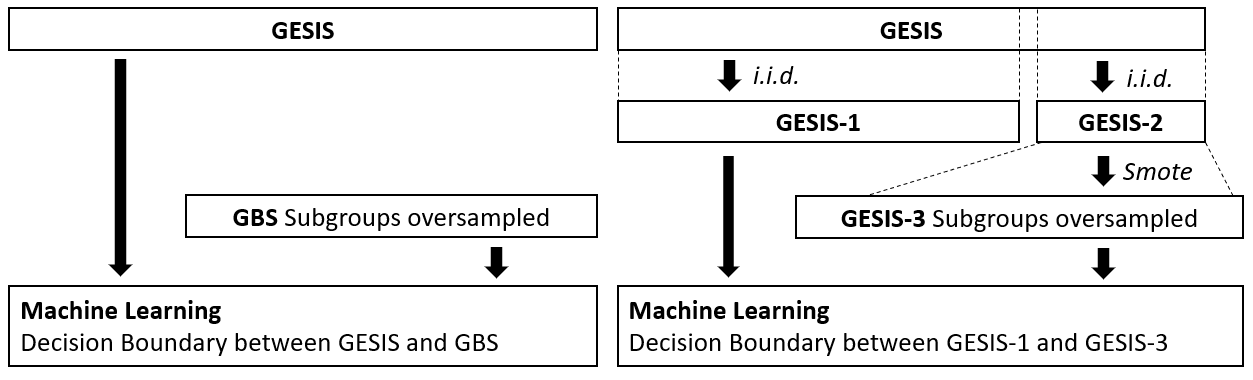
\includegraphics[scale=0.41,angle=0]{fig/procedure2}
		\label{std}
		\caption{Artificial data synthesis to overrepresent subgroups of GESIS. True negatives are removed from the MRS with positive classes GESIS (left) and GESIS-1 (right). Oversampled instances can easily be marked as such for result set comparisons.}
	\end{center}
\end{figure}

The main criteria considered in this work has been the area under the ROC curve. Having a single-number evaluation metric speeds decision-making when selecting among non-representative instances. It gives a clear preference ranking among all of them, and therefore a clear direction for progress. To enable a basis for a more informed exclusion of instances, another important performance criterion generally used in information retrieval could be added. The F-Measure, including summary statistics derived from the precision-recall curve, may be preferred to ROC curves when classes are heavily skewed \cite{jesse}. Precision and recall have been estimated in section 3.3.1 in a positive-unlabeled setting. The area under precision-recall curves \(AUPR\) can be expressed using the approximated value for the fraction of positives \(\alpha\) in \(X_u\): \(\rho = \frac{\alpha \gamma}{\hat{\eta}^{pu}}\).

